\documentclass[aspectratio=169]{beamer}


\usepackage[utf8]{inputenc}
\usepackage{amsmath}
\usepackage{amsfonts}
%\usepackage{biblatex}
\usepackage{amssymb}
\usepackage{xcolor,colortbl}
\usepackage{graphicx}
\usepackage{ragged2e}  % `\justifying` text
\usepackage{booktabs}  % Tables
\usepackage{tabularx}
\usepackage{tikz}      % Diagrams
\usetikzlibrary{calc, shapes, backgrounds}
\usepackage{amsmath}
\definecolor{Gray}{gray}{0.85}
\usepackage{amssymb}
\usepackage{subcaption}
\usepackage{dsfont}
%%\usepackage{url}       % `\url
\usepackage{listings}  % Code listings
\usepackage[T1]{fontenc}
\usepackage{filecontents}
%\usepackage[style=verbose,backend=biber]{biblatex}
%\addbibresource{bibliography.bib}
\font\myfont=cmr12 at 10pt


\usepackage{theme/beamerthemehbrs}

\author[Elanton Fernandes]{Elanton Fernandes}
\subtitle{ Active Learning Loop}
\title{Analysis of Active Learning Mechanism Applied to Language Models for Computer Assisted Short Answer Grading}
\institute[HBRS]{Hochschule Bonn-Rhein-Sieg}
\date{\today}
\subject{Test beamer}

% leave the value of this argument empty if the advisors
% should not be included on the title slide
\def\advisors{Prof. Dr. Paul G. Pl{\"o}ger, M.Sc Tim Metzler}

% \thirdpartylogo{path/to/your/image}


\begin{document}
{
\begin{frame}
\titlepage
\end{frame}
\begin{frame}{Agenda}
\tableofcontents
\end{frame}
}


\section{Motivation}
\begin{frame}{Motivation}
	In universities with an increase in number of student every semester, the number of tests conducted also increases. This means that:
	\begin{itemize}
		\item The professor spends more time in correcting student exams than preparing for lectures.
		\item If students are not assigned full scores for on a test, they expect a meaningful feedback from the professor.
	\end{itemize}
\end{frame}
\begin{frame}{Motivation}
	Consider the following dummy scenario:
	\begin{itemize}
		\item 80 students enrolled in a class.
		\item Tests are conducted bi-weekly.
		\item Professor requires 15 minutes to evaluate one student test.
		\item Total time spent by the professor to evaluate all tests per week is 10 hours. 
	\end{itemize}
\end{frame}
\section{Problem Statement}
\begin{frame}{Problem Statement}
	%\framesubtitle{Problem Statement}
	\begin{itemize}
		\item Automate the evaluation of student tests while still keeping the oracle/professor in the loop.
		\item Allow the assignment of meaningful feedback to student answers indicating their mistakes.
	\end{itemize}
	
\end{frame}

\section{State of the Art}
\begin{frame}{Related Work}
\begin{itemize}
	\item Wu et al. (2021) designed an system to assign feedback called ProtoTransformer for evaluating programming based questions but not for short text answers. It used limited number of examples \footnote{\footnotesize\tiny M. Wu, N. Goodman, C. Piech, and C. Finn, “Prototransformer: A meta-learning approach to
		providing student feedback,” 2021.}.
	
	\item Ghavidel et al. (2020) passed raw text through a transformer as input and used the output of classification model (CLS) token as feature \footnote{\footnotesize\tiny H. Ghavidel., A. Zouaq., and M. Desmarais., “Using bert and xlnet for the automatic short answer
		grading task,” in Proceedings of the 12th International Conference on Computer Supported
		Education - Volume 1: CSEDU,, pp. 58–67, INSTICC, SciTePress, 2020.}.
	
	\item Mieskes and Pado, (2018) compared score assignment between automated and human assignment for RF, SVM, and DT classifiers across multiple datasets \footnote{\footnotesize\tiny M. Mieskes and U. Pad\'o, “Work smart - reducing effort in short-answer grading,” in Proceedings of the
		7th workshop on NLP for Computer Assisted Language Learning, (Stockholm, Sweden), pp. 57–68,
		LiU Electronic Press, Nov. 2018.}.
\end{itemize}

\end{frame}

\section{Dataset}
\begin{frame}{Dataset}
\begin{table}
	\begin{tabular}{|c|c|c|c|}
		\hline
		\rowcolor{Gray}
		Dataset & Domain & No. of Question Pairs & No. of Responses\\
		\hline 
		Mohler \footnote{\footnotesize\tiny M. Mohler, R. Bunescu, and R. Mihalcea, “Learning to grade short answer questions using semantic
			similarity measures and dependency graph alignments,” June 2011.}& Computer Science& 81 & 2237 \\
		\hline
		NN Exam \footnote{\footnotesize\tiny P. G. Pl{\"o}ger, “Neural network exam dataset,” 2020.} & Neural Network \& AI & 40 & 1137 \\
		\hline
		AMR Exam \footnote{\footnotesize\tiny N. Hochgeschwender, “Autonomous mobile robots exam dataset,” 2021.}& Robotics & 5 & 190 \\
		\hline
	\end{tabular}
	\caption{Datasets used in score and feedback evaluation.}
\end{table}
\end{frame}
\section{Approach}

\begin{frame}{Approach}
\framesubtitle{Contributions}
\begin{itemize}
	\item Implement four methods to alter text for feature extraction.
	\item Implement feedback assignment for short text answers.
	\item Compare performance with five pre-trained language models and two classifiers.
\end{itemize}
\end{frame}

\begin{frame}{Approach}
	\framesubtitle{Training Cycle}
	\begin{figure}
		\centering
		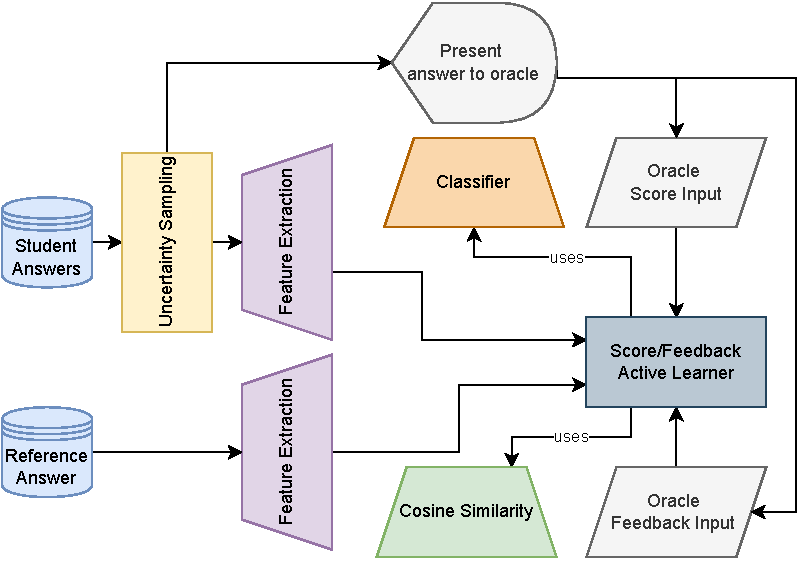
\includegraphics[scale = 0.67]{images/architecture_training.pdf}
		\label{fig:architecture train}
	\end{figure}
\end{frame}
\begin{frame}{Approach}
\framesubtitle{Prediction Cycle}
\begin{figure}
	\centering
	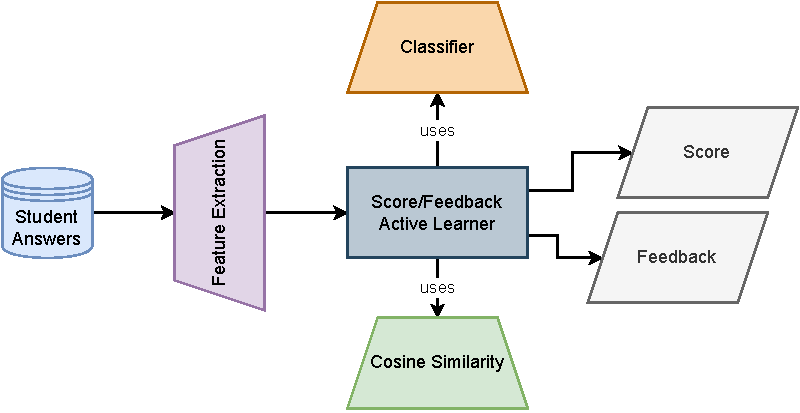
\includegraphics[scale = 0.75]{images/architecture_prediction.pdf}
	\label{fig:architecture predict}
\end{figure}
\end{frame}


\begin{frame}{Approach}
\framesubtitle{Uncertainty Sampling}
Uncertainty sampling \footnote{\footnotesize\tiny B. Settles, “Computer Sciences Department Active Learning Literature Survey,” 2009.} is a query strategy that queries the instances about which it is least certain how to label. We use uncertainty sampling variant might query the instance whose prediction is the least confident:
\begin{equation}
\label{equation:uncertainty sampling}
\scalebox{1.2}{$x_{LC} = argmin_{x} P({\hat{y}|x;\theta})$}
\end{equation}
Where $x$ is the feature, $y$ is the class label prediction, and $\hat{y} = argmax_y P({y|x;\theta})$ is the class label that has the largest posterior probability using model $\theta$.
\end{frame}
\begin{frame}{Approach}
\framesubtitle{Feature Extraction: Overview}
\begin{figure}
	\centering
	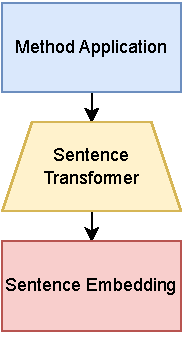
\includegraphics[scale = 0.65]{images/feature_extraction.pdf}
	\label{fig:feature extraction}
\end{figure}
\footnote{\footnotesize\tiny N. Reimers and I. Gurevych, “Sentence-bert: Sentence embeddings using siamese bert-networks,”
	2019.}
\end{frame}
\begin{frame}{Approach}
\framesubtitle{Feature Extraction: Passage-Based Method}
\begin{figure}
	\centering
	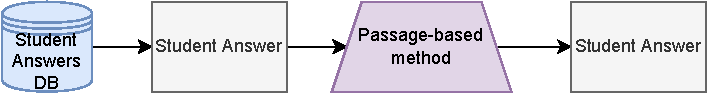
\includegraphics[scale = 1]{images/passage_FE_slides.pdf}
	\label{fig:passage fe slides}
\end{figure}
\end{frame}
\begin{frame}{Approach}
\framesubtitle{Feature Extraction: Sentence-Based Method}
\begin{figure}
	\centering
	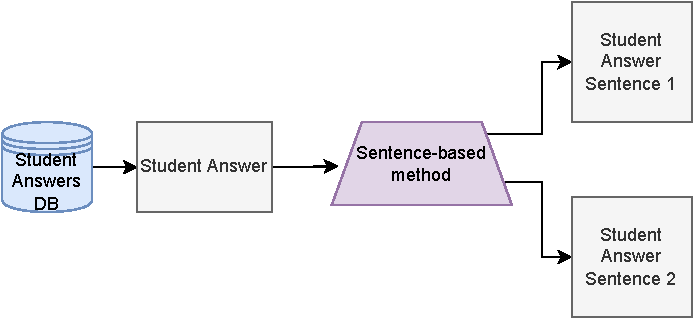
\includegraphics[scale = 1]{images/sentence_FE_slides.pdf}
	\label{fig:sentence fe slides}
\end{figure}
\end{frame}
\begin{frame}{Approach}
\framesubtitle{Feature Extraction: Chunk-Based Method}
\begin{figure}
	\centering
	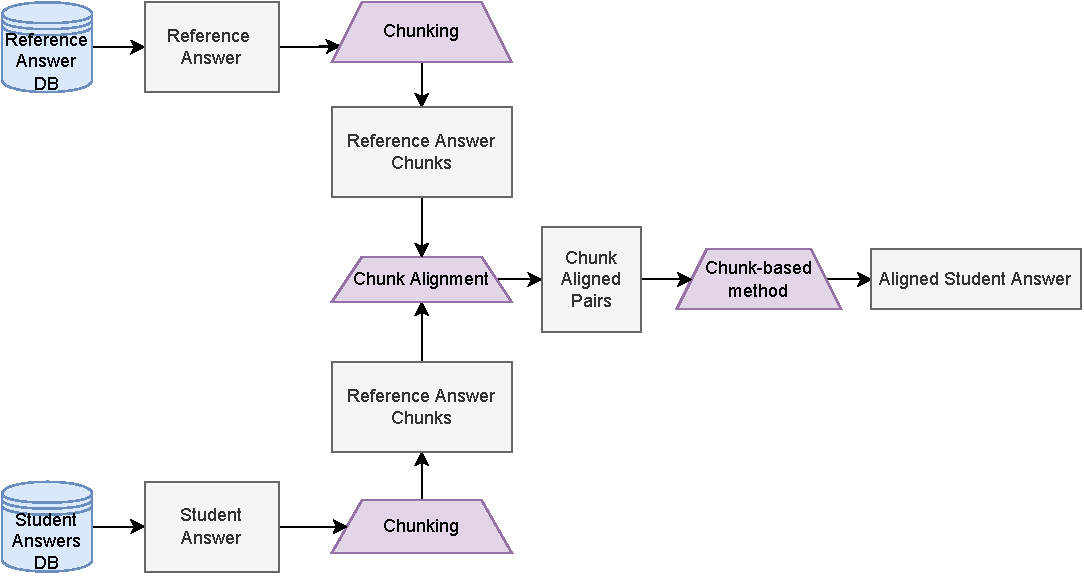
\includegraphics[scale = 0.6]{images/chunk_FE_slides.pdf}
	\label{fig:chunk fe}
\end{figure}
\end{frame}
\begin{frame}{Approach}
\framesubtitle{Feature Extraction: Resource Description Framework (RDF) Based Method}
\begin{figure}
	\centering
	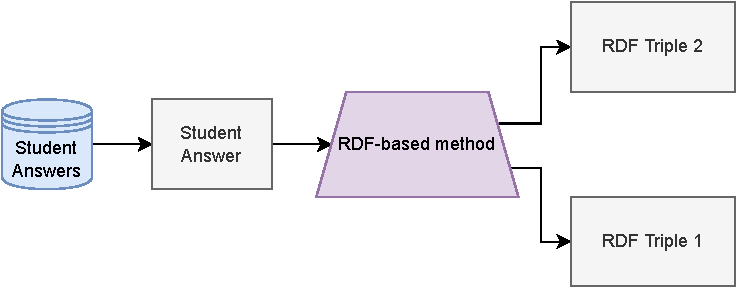
\includegraphics[scale = 1]{images/RDF_FE_slides.pdf}
	\label{fig:rdf fe}
\end{figure}
\end{frame}
\begin{frame}{Approach}
\framesubtitle{Language Models}
\begin{table}
	\begin{center}
		\begin{tabular}{ |c|c|c| }
			\hline
			Language Model \footnote{\footnotesize\tiny N. Reimers and I. Gurevych, “Sentence-bert: Sentence embeddings using siamese bert-networks,”
				2019.} & Base model & Number \\&&Training tuples  
			\\ \hline 
			all-mpnet-base-v2  & 	microsoft/mpnet-base. &1.17B
			
			\\ \hline
			all-distilroberta-v1 & 	distilroberta-base &1.12B
			\\ \hline
			all-MiniLM-L12-v2 & 		microsoft/MiniLM-L12-H384-uncased &1.17B
			\\ \hline
			multi-qa-distilbert-cos-v1 & 	distilbert-base &214M
			\\ \hline
			all-MiniLM-L6-v2 & 		nreimers/MiniLM-L6-H384-uncased &1.17B
			\\ \hline
		\end{tabular}
		\caption{Displays pre-trained language models with their base model used in training and number of training tuples used.}
		\label{table:language models}
	\end{center}
\end{table}
\end{frame}
\section{Evaluation}
\begin{frame}{Evaluation}
	\framesubtitle{Score}
	\begin{itemize}
		\item Pearsons Correlation
		\begin{equation}
		\label{equation:pearson correlation}
		\rho(y,\hat{y}) = \frac{cov(\vec{y},\hat{\vec{y}})}{\sigma_y \sigma_{\hat{y}}}
		\end{equation}
		\item RMSE Score
		\begin{equation}
		\label{equation:Root mean square error}
		RMSE = \sqrt{\frac{1}{n}\Sigma_{i=1}^n(\hat{\vec{y_i}} - \vec{y}_i)^2}
		\end{equation}
	\end{itemize}
Where $\vec{y}$ represents actual grade and $\hat{\vec{y}}$ represents predicted grade with $\sigma_y$ and $\sigma_{\hat{y}}$ computed as the standard deviation of $\vec{y}$ and $\hat{\vec{y}}$
\end{frame}
\begin{frame}{Evaluation}
\framesubtitle{Feedback}
\begin{table}
	\begin{center}
		\begin{tabular}{ |c|c| }
			\hline
			\cellcolor{Gray}Question & \cellcolor{Gray}What is a variable?  
			\\ \hline 
			Reference Answer & A location in memory that can store a value.
			\\ \hline
			\cellcolor{Gray}Student Answer & \cellcolor{Gray}A value/word that can assume any of a set of values
			\\ \hline
			Feedback A & Correct
			\\ \hline
			\cellcolor{Gray}Feedback B & \cellcolor{Gray}Missing keywords: Location in memory
			\\ \hline
			Feedback C & A variable is a location in memory that stores a value
			\\ \hline
		\end{tabular}
		\caption{Presented survey to participants.}
		\label{table:language models}
	\end{center}
\end{table}
\centering
$Agreement\ Score$ $= \frac{Model\ generated\ most\ rated\ feedback}{Total\ Number\ of\ Participants}\times 100$
\end{frame}
\section{Results}
\begin{frame}{Results}
	\framesubtitle{Notations}
	\begin{columns}
		\begin{column}{0.5\textwidth}
			\begin{table}
				\centering
				\begin{tabular}{|c|c|}
					\hline
					\rowcolor{Gray}
					Method & Notation\\
					\hline
					Passage-based Methods & M1\\
					\hline
					Sentence-based Method & M2\\
					\hline
					Chunk-based Method & M3\\
					\hline
					RDF-based Method & M4\\
					\hline
				\end{tabular}
			\end{table}
		\end{column}
	\begin{column}{0.5\textwidth}
		\begin{table}
			\centering
			\begin{tabular}{|c|c|}
				\hline
				\rowcolor{Gray}
				Language Model & Notation\\
				\hline
				all-mpnet-base-v2 & LM1\\
				\hline
				all-distilroberta-v1 & LM2\\
				\hline
				all-MiniLM-L12-v2 & LM3\\
				\hline
				multi-qa-distilbert-cos-v1 & LM4\\
				\hline
				all-MiniLM-L6-v2 & LM5\\
				\hline
				
			\end{tabular}
		\end{table}
	\end{column}
	\end{columns}
	
\end{frame}
\begin{frame}{Results}
	\framesubtitle{Score: Pearson Correlation (Methods)}
\begin{table}
	\centering
	\begin{subtable}[c]{0.6\textwidth}
		
		\begin{tabular}{|c|c|c|c|c|}
			\hline
			Dataset & M1 & M2 & M3 & M4 \\
			\hline
			Mohler  & \underline{\textbf{0.826}}  &\textbf{0.791} &\textbf{0.816} &0.782 \\
			\hline
			NN Exam  &\underline{\textbf{0.941}} &\textbf{0.828} &0.561 &\textbf{0.846} \\
			\hline
			AMR Exam  &\underline{\textbf{0.658}} &0.458 &\textbf{0.640} & \textcolor{gray}{0.428} \\
			\hline
		\end{tabular}
		\subcaption{}
	\end{subtable}
\centering
	\begin{subtable}[c]{0.6\textwidth}
		
		\begin{tabular}{|c|c|c|c|c|}
			\hline
			Dataset & M1 & M2 & M3 & M4 \\
			\hline
			Mohler &0.689  &0.627 &0.687 &\textbf{0.792} \\
			\hline
			NN Exam &0.889 &0.791 &\textbf{0.638} &0.664 \\
			\hline
			AMR Exam &0.622 &\textbf{0.474} &0.593 &\textcolor{gray}{0.428} \\
			\hline
		\end{tabular}	
		\subcaption{}
	\end{subtable}
	\caption{Comparison of Pearson Correlation between Random Forest (a) and AdaBoost (b) classifiers. Where M1: Passage-based, M2: Sentence-based, M3:Chunk-based, and M4: RDF-based method.}
\end{table}
\end{frame}

\begin{frame}{Results}
\framesubtitle{Score: Pearson Correlation (Language Models)}
\noindent
\begin{table}
	\noindent
	\begin{subtable}[c]{0.7\textwidth}
		\noindent
		\centering
		\begin{tabular}{|c|c|c|c|c|c|}
			\hline
			Dataset & LM1 & LM2 & LM3 & LM4 & LM5 \\
			\hline
			Mohler &\underline{\textbf{0.802}}& \textbf{0.797}& \textbf{0.796}& \textbf{0.796}& \textbf{0.789}\\
			\hline
			NN Exam &\textbf{0.732}& \textbf{0.670}& \textbf{0.705}& \textbf{0.755}& \underline{\textbf{0.760}}\\
			\hline
			AMR Exam &0.453& \textbf{0.518}& \underline{\textbf{0.525}}& \textbf{0.523}& \textbf{0.503}\\
			\hline
		\end{tabular}
		\subcaption{}
	\end{subtable}
	\begin{subtable}[c]{0.7\textwidth}
		\centering
		\begin{tabular}{|c|c|c|c|c|c|}
			\hline
			Dataset & LM1 & LM2 & LM3 & LM4 & LM5 \\
			\hline
			Mohler &0.659& 0.673& 0.211& 0.544& 0.499 \\
			\hline
			NN Exam &0.614& 0.653& 0.704& 0.698& 0.605\\
			\hline
			AMR Exam &\textbf{0.502}& 0.440& 0.430& 0.508& 0.467\\
			\hline
		\end{tabular}	
		\subcaption{}
	\end{subtable}
	\caption{Comparison of Pearson Correlation between Random Forest (a) and AdaBoost (b) classifiers with language models (LM).}
\end{table}
\end{frame}


%Rmse
\begin{frame}{Results}
\framesubtitle{Score: Root Mean Square Error (Methods)}
\begin{table}
	\begin{subtable}[c]{0.6\textwidth}
		\centering
		\begin{tabular}{|c|c|c|c|c|}
			\hline
			Dataset & M1 & M2 & M3 & M4 \\
			\hline
			Mohler & \underline{\textbf{0.893}}  &\textbf{0.949} &\textbf{0.920} &0.942 \\
			\hline
			NN Exam &\underline{\textbf{0.296}} &\textbf{0.520} &\textbf{0.433} &\textbf{0.522} \\
			\hline
			AMR Exam &\underline{\textbf{0.596}} &0.716 &\underline{\textbf{0.596}} & \textbf{0.736} \\
			\hline
		\end{tabular}
		\subcaption{}
	\end{subtable}
	\begin{subtable}[c]{0.6\textwidth}
		\centering
		\begin{tabular}{|c|c|c|c|c|}
			\hline
			Dataset & M1 & M2 & M3 & M4 \\
			\hline
			Mohler &1.218  &1.226 &1.169 &\textbf{0.920} \\
			\hline
			NN Exam &0.405 &0.571 &{0.495} &0.741 \\
			\hline
			AMR Exam &0.616 &\textbf{0.707} &0.630 &{0.741} \\
			\hline
		\end{tabular}	
		\subcaption{}
	\end{subtable}
	\caption{Comparison of RMSE score between Random Forest (a) and AdaBoost (b) classifiers with methods (M).}
\end{table}
\end{frame}

\begin{frame}{Results}
\framesubtitle{Score: Root Mean Square Error (Language Models)}
\begin{table}
\begin{subtable}[c]{0.7\textwidth}
	\centering
	\begin{tabular}{|c|c|c|c|c|c|}
		\hline
		Dataset & LM1 & LM2 & LM3 & LM4 & LM5 \\
		\hline
		Mohler &\underline{\textbf{0.931}}& \textbf{0.941}& \textbf{0.941}& \textbf{0.941}& \textbf{0.956}\\
		\hline
		NN Exam &\underline{\textbf{0.484}}& {0.591}& \textbf{0.558}& \textbf{0.490}& \textbf{0.492}\\
		\hline
		AMR Exam &0.735& \textbf{0.680}& \underline{\textbf{0.676}}& 0.684& \textbf{0.698}\\
		\hline
	\end{tabular}
	\subcaption{}
\end{subtable}
\begin{subtable}[c]{0.7\textwidth}
	\centering
	\begin{tabular}{|c|c|c|c|c|c|}
		\hline
		Dataset & LM1 & LM2 & LM3 & LM4 & LM5 \\
		\hline
		Mohler &1.182& 1.163& 1.667& 1.278& 1.363 \\
		\hline
		NN Exam &0.632& \textbf{0.582}& 0.587& 0.587& 0.650\\
		\hline
		AMR Exam &\textbf{0.692}& 0.748& 0.718& \textbf{0.682}& 0.736\\
		\hline
	\end{tabular}	
	\subcaption{}
\end{subtable}
\caption{Comparison of RMSE score between Random Forest (a) and AdaBoost (b) classifiers with language models (LM).}
\end{table}
\end{frame}
%Feedbacks
\begin{frame}{Results}
	\framesubtitle{Feedback: Survey Results}
	\begin{columns}
		\begin{column}{0.65\textwidth}
		\begin{table}
			\begin{tabular}{ |c|c| }
				\hline
				Question & What is a variable?  
				\\ \hline 
				Reference Answer & A location in memory\\& that can store a value.
				\\ \hline
				Student Answer & A value/word that can\\& assume any of a set of values
				\\ \hline
				Feedback A & Correct
				\\ \hline
				Feedback B & Missing keywords:\\& Location in memory
				\\ \hline
				Feedback C & A variable is a location\\& in memory that stores a value
				\\ \hline
			\end{tabular}
		\end{table}
	\end{column}
	\begin{column}{0.5\textwidth}
		\begin{center}
			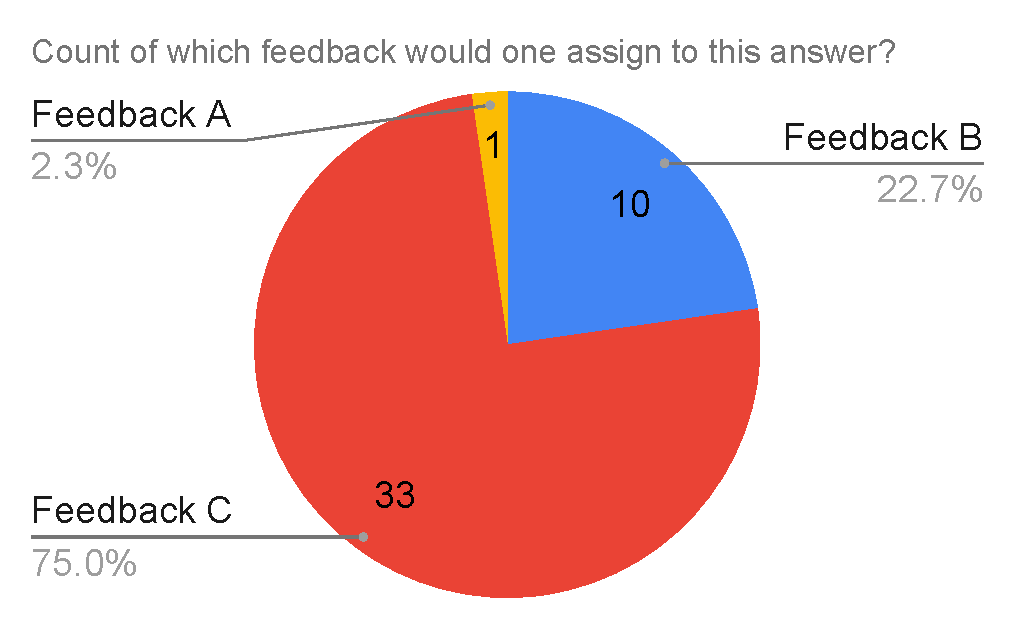
\includegraphics[width=1\textwidth]{images/survey_1.pdf}
		\end{center}
	\end{column}
	\end{columns}
\end{frame}
\begin{frame}{Results}
	\framesubtitle{Feedback: Agreement Scores (Methods)}
	\begin{columns}
		\begin{column}{1\textwidth}
	\begin{table}
			\centering
			\begin{tabular}{|c|c|c|c|c|}
				
				\hline
				\rowcolor{Gray}
				Classifier&\multicolumn{4}{|c|}{Methods}\\
				\hline
				 & M1 & M2 & M3 & M4 \\
				\hline
				Random Forest &\textbf{60.00}&22.73&31.82&35.91\\
				\hline
				AdaBoost &\textbf{60.00}&22.73&31.82&35.91\\
				\hline
			\end{tabular}
		
		\caption{Mean agreement scores for Random Forest (a) and AdaBoost classifier (b) with methods.}
	\end{table}
\end{column}
\end{columns}
\end{frame}
\begin{frame}{Results}
	\framesubtitle{Feedback: Agreement Scores (Models)}
	\begin{table}
			\centering
			\begin{tabular}{|c|c|c|c|c|c|}
				
			\hline
			\rowcolor{Gray}
			Classifier&\multicolumn{5}{|c|}{Language Models}\\
			\hline
			 & LM1 & LM2 & LM3 & LM4 & LM5 \\
			\hline
			Random Forest &25.11& 26.82& 24.66& \textbf{37.05}& 21.25\\
			\hline
			AdaBoost &25.11& 26.82& 24.66& \textbf{37.05}& 21.25\\
			\hline
			\end{tabular}
		\caption{Mean agreement scores for Random Forest and AdaBoost classifier with Language Models.}
	\end{table}
	
\end{frame}
\begin{frame}{Results}
	\framesubtitle{Summary: Scores}
	\begin{table}
	\begin{subtable}[c]{0.7\textwidth}
				\centering
				\begin{tabular}{|c|c|c|c|}
					\hline
					Dataset & Method & Model & Classifier \\
					\hline
					Mohler & M1 & LM1& Random Forest \\
					\hline
					NN Exam & M1 & LM5 & Random Forest\\
					\hline
					AMR Exam & M1& LM3 & Random Forest\\
					\hline	
				\end{tabular}
			\subcaption{}
			\end{subtable}
		\begin{subtable}[c]{0.7\textwidth}
			
			\centering
			\begin{tabular}{|c|c|c|c|}
				\hline
				Dataset & Method & Model & Classifier \\
				\hline
				Mohler & M1 & LM1& Random Forest \\
				\hline
				NN Exam & M1 & LM1 & Random Forest\\
				\hline
				AMR Exam & M1\& M3 & LM3 & Random Forest\\
				\hline	
			\end{tabular}
			\subcaption{}
		\end{subtable}
	\caption{Performance summary Pearson correlation (a) and RMSE score (b)}
\end{table}
\end{frame}

\begin{frame}{Results}
	\framesubtitle{Feedback}
	\begin{table}
		\centering
		\begin{tabular}{|c|c|c|c|c|}
			\hline
			Dataset & Method & Model & Method-Model & Classifier \\
			\hline
			Mohler & M1 & LM4 & M1-LM4 & Random Forest \\
			\hline
		\end{tabular}
	\caption{Results of feedback evaluation}
	\end{table}
\end{frame}
\section{Summary}
\begin{frame}{Summary}
	\begin{itemize}
		\item Four methods implemented to alter student answer text.
		\item Designed system that keeps oracle in training loop.
		\item System allows assignment of feedback.
		\item Pearson correlation and RMSE score used as score evaluation metrics.
		\item Survey created and used in the evaluation of the feedback assigned by the model.
	\end{itemize}
\end{frame}
\section{Future Work}
\begin{frame}{Future Work}
\begin{itemize}
	\item RDF-based method did not give good RDF triplets. Fine tune model for better results.
	\item Fine tune language models similar to \textcolor{blue}{multi-qa-distilbert-cos-v1} to create embeddings.
	\item Chunk-based Method took 41 sec per prediction. This time needs to be reduced.
\end{itemize}
\end{frame}
\begin{frame}

\end{frame}



%    \begin{frame}[label=bibliography]{References}
%      \begin{thebibliography}{9}
%      	\bibitem{SBERT}
%      		Reimers, Nils and Gurevych, Iryna ``Sentence-BERT: Sentence Embeddings using Siamese BERT-Networks'', 2019.
%      		
%        \bibitem{mohler}
%            M. Mohler, R. Bunescu, and R. Mihalcea, “Learning to grade short answer questions using semantic
%            similarity measures and dependency graph alignments,” in Proceedings of the 49th Annual Meeting of
%            the Association for Computational Linguistics: Human Language Technologies, (Portland, Oregon,
%            USA), pp. 752–762, Association for Computational Linguistics, June 2011.
%        \bibitem{lamport94}
%            Leslie~Lamport.
%            \emph{\LaTeX : A Document Preparation System}.
%            Addison-Wesley, 1986.
%        \bibitem{MG94}
%            M.~Goossens, F.~Mittelbach, and A.~Samarin.
%            \emph{The \LaTeX\ Companion}.
%            Addison-Wesley, 1994.
%        \bibitem{tantau04}
%            Till~Tantau.
%            \emph{User's Guide to the Beamer Class Version 3.01}.
%            Available at \url{http://latex-beamer.sourceforge.net}.
%        \bibitem{MS05}
%            A.~Mertz and W.~Slough.
%            Edited by B.~Beeton and K.~Berry.
%            \emph{Beamer by example} In TUGboat,
%              Vol. 26, No. 1., pp. 68-73.
%      \end{thebibliography}
%    \end{frame}

\begin{frame}{Foundation}
\framesubtitle{Cosine Similarity}

If $\boldsymbol{x}$ and $\boldsymbol{y}$ are two sentences and  $\boldsymbol{e_x}$ and $\boldsymbol{e_y}$ are embeddings of these sentences. Then the cosine similarity is given by:

\begin{equation}
\label{equation:cosinesimilarity}
S_{cosine}(\boldsymbol{e_x},\boldsymbol{e_y}) = \frac{\boldsymbol{e_x} \cdot \boldsymbol{e_y}}{\|\boldsymbol{e_x}\| \|\boldsymbol{e_y}\|}
\end{equation}

\end{frame}
\begin{frame}{Foundation}
\framesubtitle{Active Learning}
\begin{figure}
	\centering
	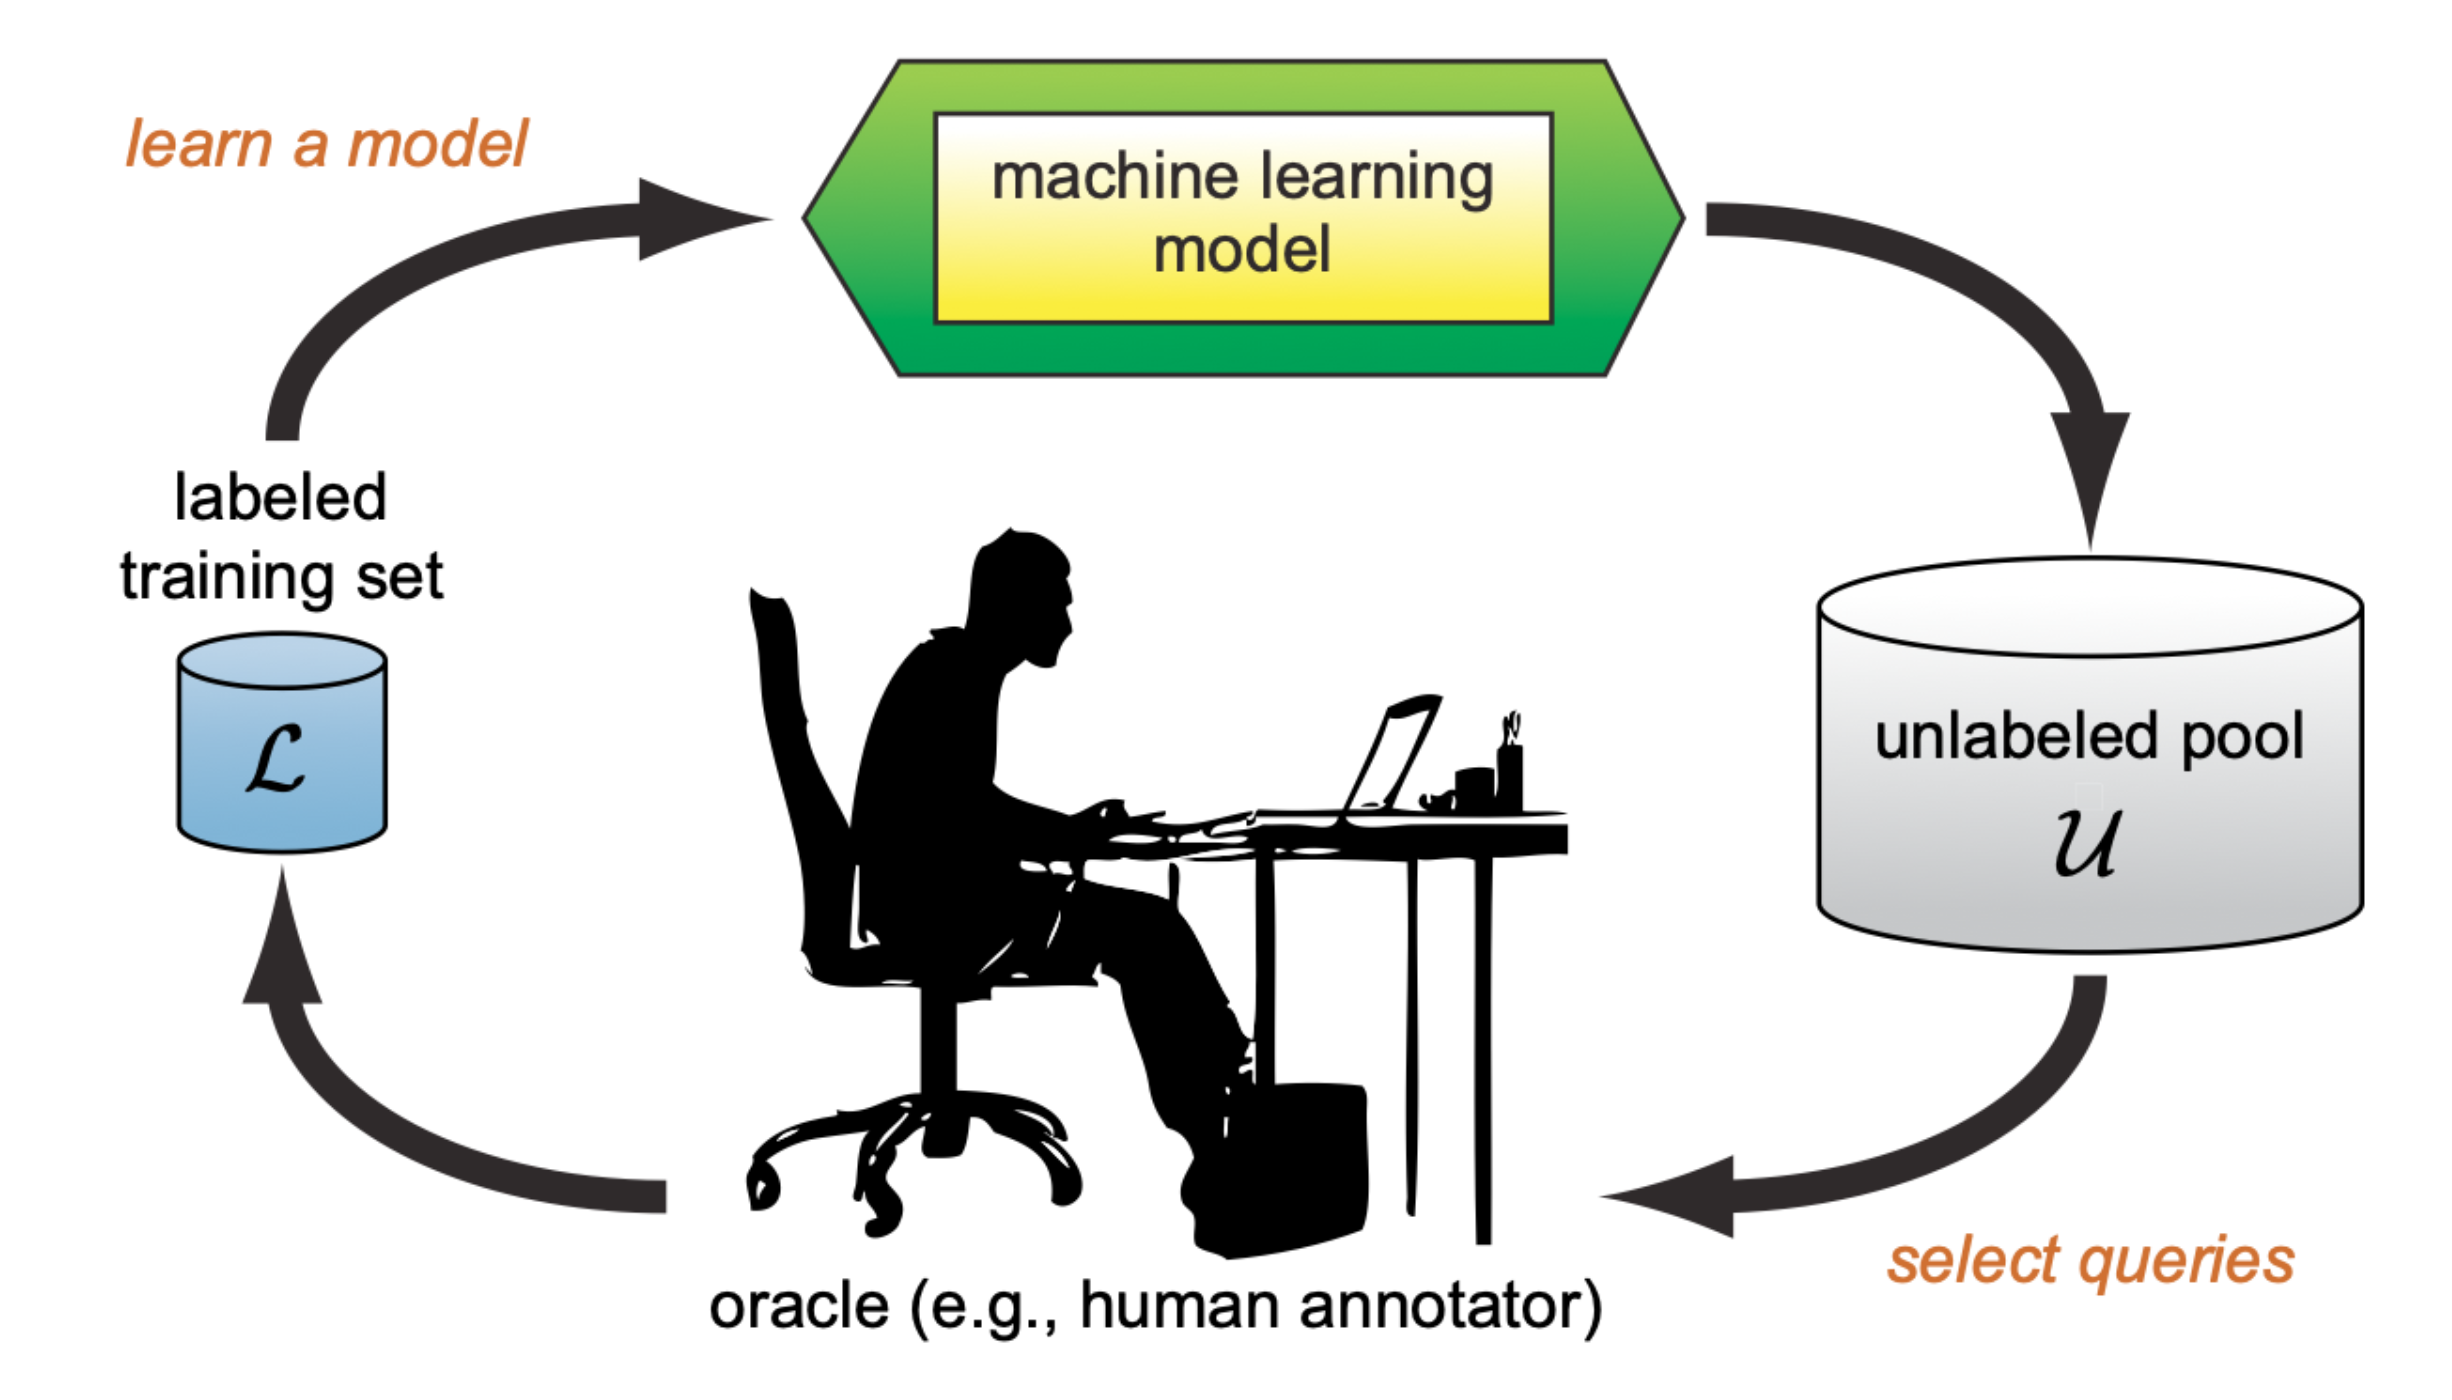
\includegraphics[scale = 0.25]{images/activelearningloopSettles.png}
	\label{fig:passage fe}
\end{figure}
\end{frame}
\begin{frame}{Foundation}
	\framesubtitle{Chunking}
	\begin{figure}
		\centering
		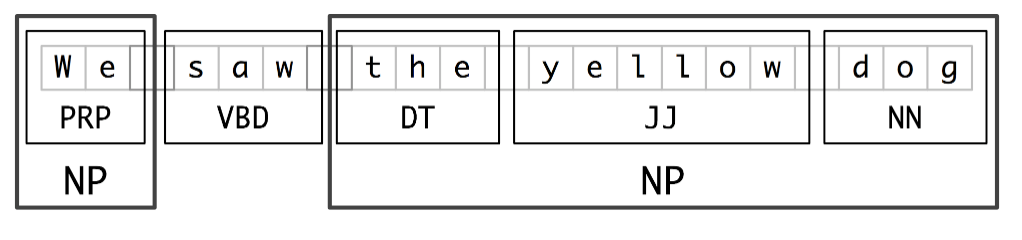
\includegraphics[scale = 0.5]{images/chunking.png}
		\label{fig:passage fe}
	\end{figure}
\begin{table}
	\centering
	\resizebox{0.8\textwidth}{!}{%
	\begin{tabular}{|c|c|c|c|}
		\hline
		\textbf{Symbol} & \textbf{Meaning} & \textbf{Symbol} &\textbf{Meaning}\\
		\hline
		\cellcolor{Gray}NP & \cellcolor{Gray}Noun Phrase & VP &Verb phrase \\
		\hline
		NN & Noun & \cellcolor{Gray}DT & \cellcolor{Gray}zero or one determiner
		\\ \hline
		\cellcolor{Gray}JJ & \cellcolor{Gray}One or more adjectives &PRP& Preposition
		
		\\ \hline
		
	\end{tabular}}
\end{table}
\end{frame}
\begin{frame}{Approach:Example}
\framesubtitle{Feature Extraction: Passage-based method}
\begin{figure}
\centering
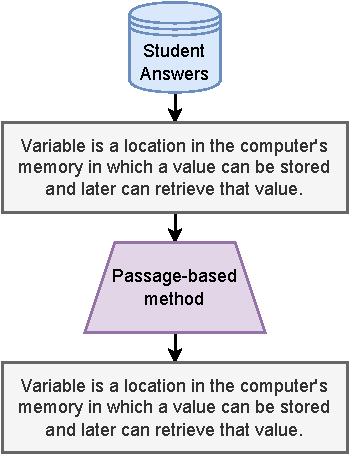
\includegraphics[scale = 0.65]{images/passage_FE.pdf}
\label{fig:passage fe}
\end{figure}
\end{frame}
\begin{frame}{Approach}
\framesubtitle{Feature Extraction: Sentence-based method}
\begin{figure}
\centering
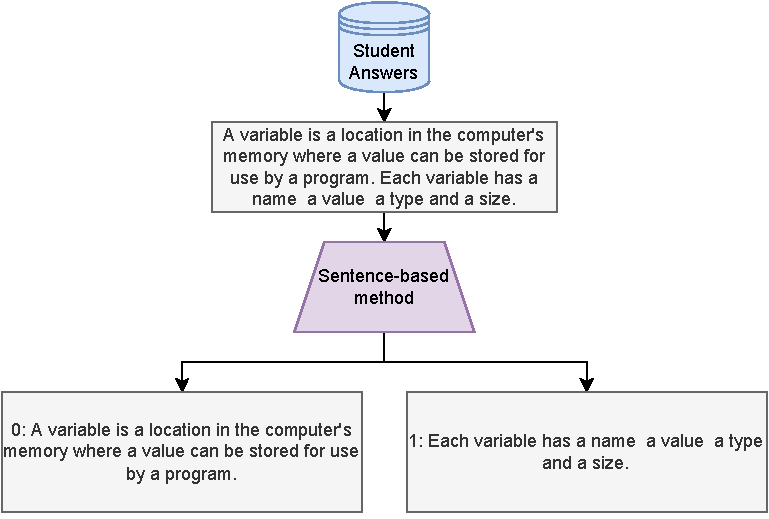
\includegraphics[scale = 0.65]{images/sentence_FE.pdf}
\label{fig:sentence fe}
\end{figure}
\end{frame}
\begin{frame}{Approach}
\framesubtitle{Feature Extraction: Chunk-based method}
\begin{figure}
\centering
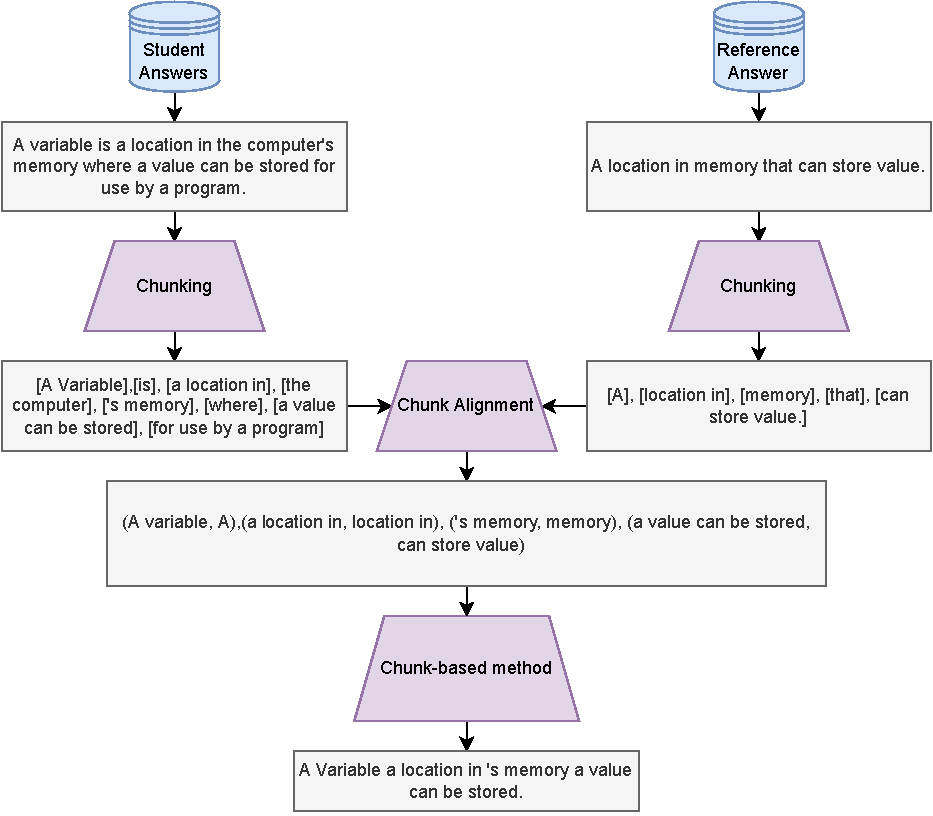
\includegraphics[scale = 0.5]{images/chunk_FE.pdf}
\label{fig:chunk fe}
\end{figure}
\end{frame}
\begin{frame}{Approach}
\framesubtitle{Feature Extraction: RDF-based method}
\begin{figure}
\centering
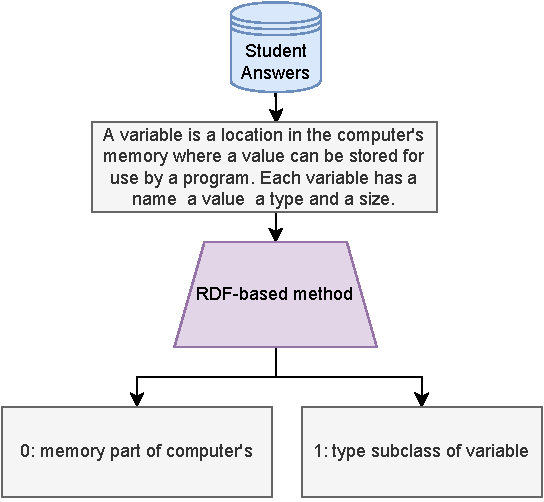
\includegraphics[scale = 0.65]{images/RDF_FE.pdf}
\label{fig:rdf fe}
\end{figure}
\end{frame}

\begin{frame}{Results}
\framesubtitle{Feedback: Survey Results}
		\begin{table}
			\resizebox{\textwidth}{!}{%
			\begin{tabular}{ |c|l| }
				\hline
				Question & What stages of the software lifecycle are influenced by the testing stage  
				\\ \hline 
				Reference Answer & The testing stage can influence both the coding stage (phase 5) and the\\& solution refinement stage (phase 7)
				\\ \hline
				Student Answer & All stages are influenced except setting the program requirements. If a test\\& fails it can change the whole design implementation etc of a program\\& as well as the final outcome.
				\\ \hline
				Feedback A & The testing phase affects the coding/production phase and the refinement/maintenance phase
				\\ \hline
				Feedback B & Correct
				\\ \hline
				Feedback C & Missing keywords: Refinement stage,Coding phase
				\\ \hline
			\end{tabular}}
		\end{table}
\end{frame}
\begin{frame}
		\begin{center}
			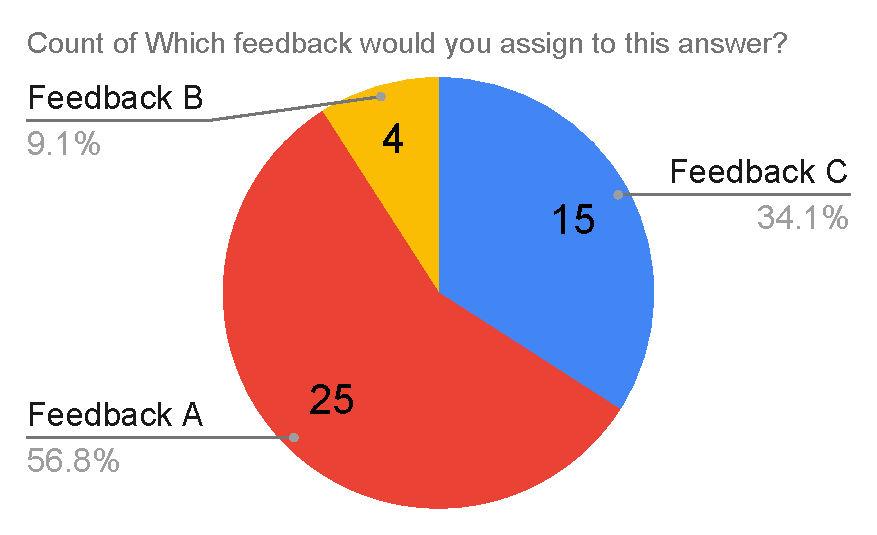
\includegraphics[width=0.9\textwidth]{images/survey_3.pdf}
		\end{center}
\end{frame}

\begin{frame}{Results}
\framesubtitle{Feedback: Survey Results}
\begin{table}
	\resizebox{\textwidth}{!}{%
	\begin{tabular}{ |c|l| }
		\hline
		Question &What are the main advantages associated with object oriented programming?
		\\ \hline 
		Reference Answer & Abstraction and reusability.
		\\ \hline
		Student Answer & Re-usability  and ease of maintenance
		\\ \hline
		Feedback A & Missing keywords: Reusability, Abstraction
		\\ \hline
		Feedback B & Correct
		\\ \hline
		Feedback C & The main advantages of OOP are abstraction and reusability
		\\ \hline
		Feedback D & Encapsulation is similar to abstraction but not the same and second advantage is reusability.
		\\ \hline
	\end{tabular}}
\end{table}
\end{frame}
\begin{frame}
\begin{center}
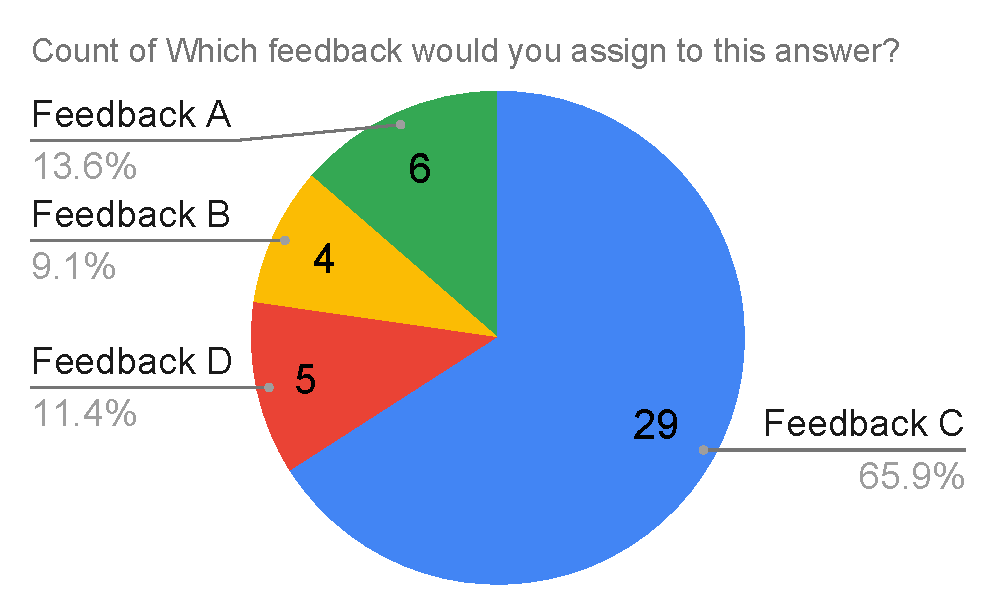
\includegraphics[width=0.9\textwidth]{images/survey_2.pdf}
\end{center}
\end{frame}


\begin{frame}{Results}
\framesubtitle{Feedback: Survey Results}
\begin{table}
	\begin{tabular}{ |c|c| }
		\hline
		Question & What is a variable?  
		\\ \hline 
		Reference Answer & A location in memory\\& that can store a value.
		\\ \hline
		Student Answer & a value/word that can\\& assume any of a set of values
		\\ \hline
		Feedback A & correct
		\\ \hline
		Feedback B & missing keywords:\\& location in memory
		\\ \hline
		Feedback C & A variable is a location\\& in memory that stores a value
		\\ \hline
	\end{tabular}
\end{table}
\end{frame}
\begin{frame}
\begin{center}
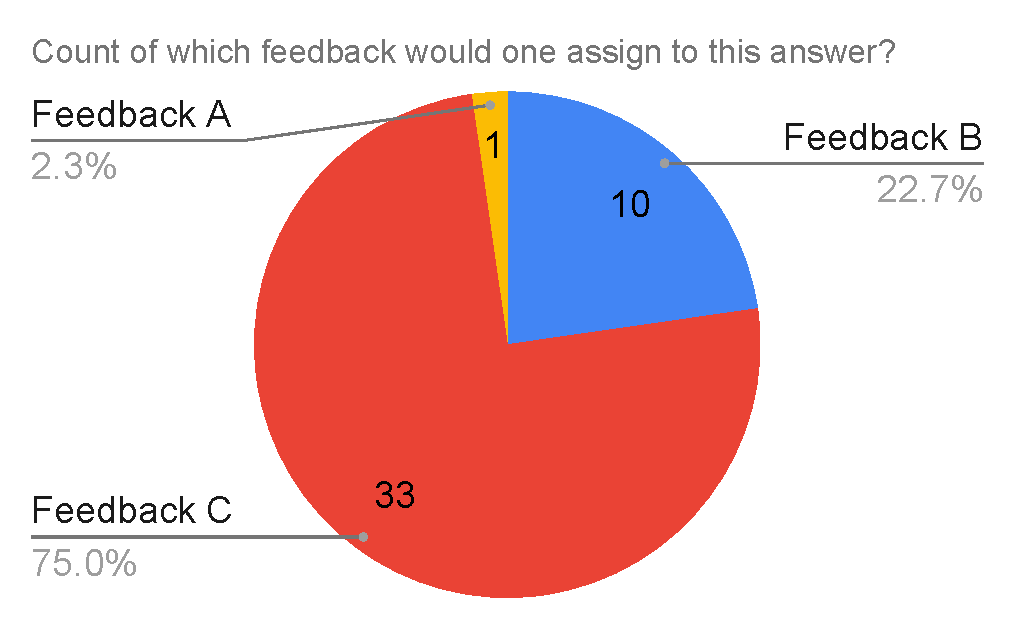
\includegraphics[width=0.9\textwidth]{images/survey_1.pdf}
\end{center}
\end{frame}


\begin{frame}{Results}
\framesubtitle{Feedback: Survey Results}
\begin{table}
	\resizebox{0.8\textwidth}{!}{%
	\begin{tabular}{ |c|l| }
		\hline
		Question & What is the difference between a constructor and a function?
		\\ \hline 
		Reference Answer & A constructor is called whenever an object is created \\& whereas a function needs to be called explicitly.\\& Constructors do not have return type  but functions have\\& to indicate a return type.
		\\ \hline
		Student Answer & Constructors don't have a return type.
		\\ \hline
		Feedback A & Missing point: A constructor is called whenever\\& an object is created  whereas a function needs\\& to be called explicitly.
		\\ \hline
		Feedback B & Correct
		\\ \hline
		Feedback C & Missing point: Constructors do not have return\\& type  but functions have to indicate a return type.
		\\ \hline
		Feedback D & Answer not explained properly. Information on\\& function/ constructor calling and their return type missing.
		\\ \hline
	\end{tabular}}
\end{table}
\end{frame}
\begin{frame}
\begin{center}
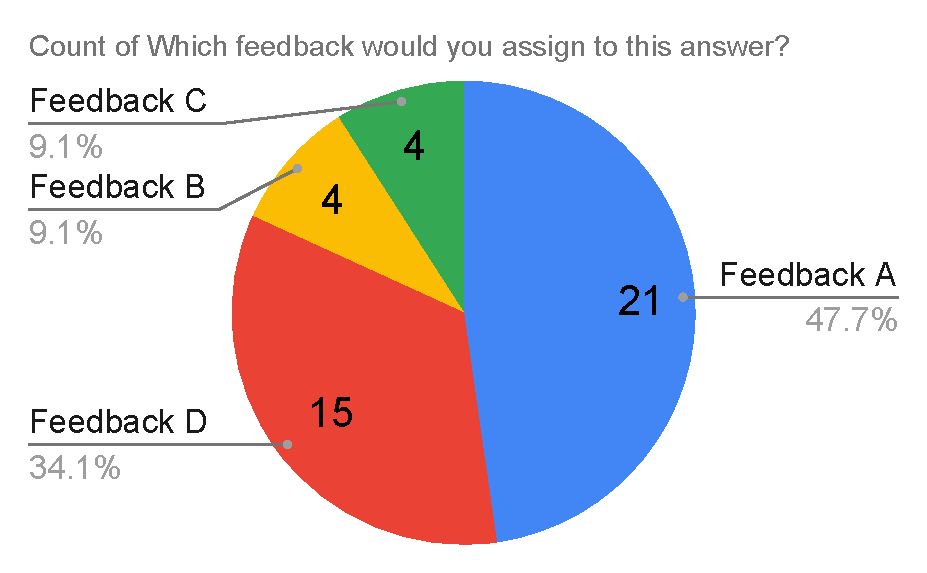
\includegraphics[width=0.9\textwidth]{images/survey_4.pdf}
\end{center}
\end{frame}


\begin{frame}{Results}
\framesubtitle{Feedback: Survey Results}
\begin{table}
	\resizebox{0.8\textwidth}{!}{%
		\begin{tabular}{ |c|l| }
			\hline
			Question & When does C++ create a default constructor?
			\\ \hline 
			Reference Answer & If no constructor is provided  the compiler\\& provides one by default. If a constructor is\\& defined for a class  the compiler does not\\& create a default constructor.
			\\ \hline
			Student Answer & When non are provided
			\\ \hline
			Feedback A & If no constructor is defined then a default\\& constructor is created during compilation.
			\\ \hline
			Feedback B & Missing keywords: during compilation
			\\ \hline
			Feedback C & Correct
			\\ \hline
	\end{tabular}}
\end{table}
\end{frame}
\begin{frame}
\begin{center}
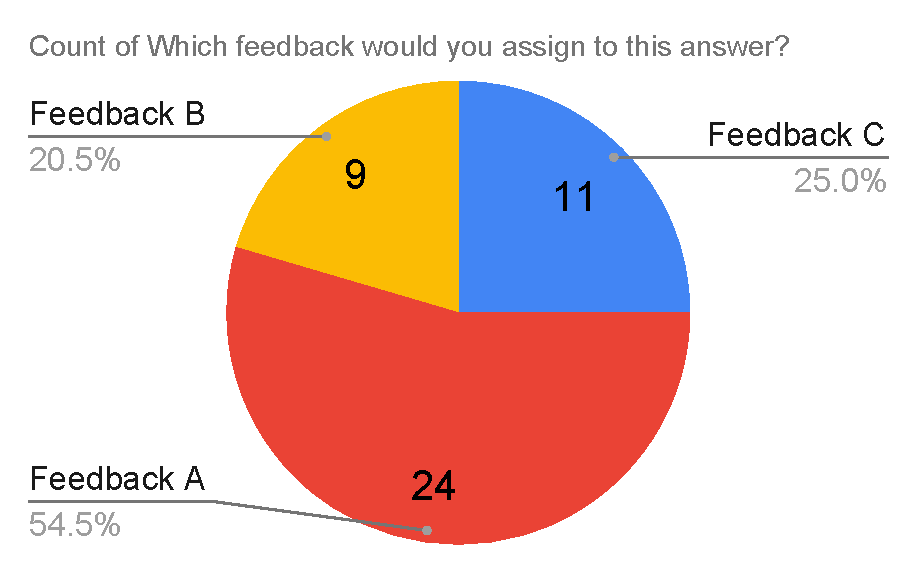
\includegraphics[width=0.9\textwidth]{images/survey_5.pdf}
\end{center}
\end{frame}
\begin{frame}{Results}
\framesubtitle{Prediction Time}
	\begin{table}
		\begin{center}
			\begin{tabular}{ |c|c| }
				\hline
				\textbf{Method} & \textbf{Avg. Prediction Time (sec)}
				\\ \hline
				Passage-Based & \textbf{0.0344}
				\\ \hline
				Sentence-Based & 0.0749
				\\ \hline
				Chunk-Based & 41.3039
				\\ \hline
				RDF-Based & 5.8424
				\\ \hline
				
			\end{tabular}
			\caption{Shows average prediction time (in seconds) per response for each method.}
			\label{table:prediction time}
		\end{center}
	\end{table}
\end{frame}
%\begin{frame}{Jabberwocky}
%      \framesubtitle{Lewis Carroll}%
%      \begin{tikzpicture}[overlay,remember picture]
%        \node[anchor=south east,xshift=-30pt,yshift=35pt]
%          at (current page.south east) {
%            %\includegraphics[width=35mm]{resources/jabberwocky-light}
%          };
%      \end{tikzpicture}%
%      'Twas brillig, and the slithy toves\\
%      Did gyre and gimble in the wabe;\\
%      All mimsy were the borogoves,\\
%      And the mome raths outgrabe.\\\bigskip
%
%      “Beware the Jabberwock, my son!\\
%      The jaws that bite, the claws that catch!\\
%      Beware the Jubjub bird, and shun\\
%      The frumious Bandersnatch!”\\
%\end{frame}
%
%
%\begin{frame}[label=lists]{Lists and locales}
%      \framesubtitle{Lorem ipsum dolor sit amet}
%      \begin{columns}[onlytextwidth]
%        \column{.5\textwidth}
%          \begin{itemize}
%            \item Nulla nec lacinia odio. Curabitur urna tellus.
%            \begin{itemize}
%              \item Fusce id sodales dolor. Sed id metus dui.
%              \begin{itemize}
%                \item Cupio virtus licet mi vel feugiat.
%              \end{itemize}
%            \end{itemize}
%          \end{itemize}
%        \column{.5\textwidth}
%          \begin{enumerate}
%            \item Donec porta, risus porttitor egestas scelerisque video.
%            \begin{enumerate}
%              \item Nunc non ante fringilla, manus potentis cario.
%              \begin{enumerate}
%                \item Pellentesque servus morbi tristique.
%              \end{enumerate}
%            \end{enumerate}
%          \end{enumerate}
%      \end{columns}
%      \bigskip
%      \justifying
%
%      {\uselanguage{czech}Nechť již hříšné saxofony ďáblů
%      rozzvučí síň úděsnými tóny waltzu, tanga a quickstepu!}
%      {\uselanguage{slovak} Nezvyčajné kŕdle šťastných figliarskych
%      ďatľov učia pri kótovanom ústí Váhu mĺkveho koňa Waldemara
%      obžierať väč\-šie kusy exkluzívnej kôry.}
%      {\uselanguage{english}The quick, brown fox jumps over a lazy
%      dog. DJs flock by when MTV ax quiz prog. “Now fax quiz Jack!”}
%\end{frame}
%
%\subsection{Structuring Elements}
%    \begin{frame}[label=simmonshall]{Text blocks}
%      \framesubtitle{In plain, example, and \alert{alert} flavour}
%      \alert{This text} is highlighted.
%
%      \begin{block}{A plain block}
%        This is a plain block containing some \alert{highlighted text}.
%      \end{block}
%      \begin{exampleblock}{An example block}
%        This is an example block containing some \alert{highlighted text}.
%      \end{exampleblock}
%      \begin{alertblock}{An alert block}
%        This is an alert block containing some \alert{highlighted text}.
%      \end{alertblock}
%    \end{frame}
%
%
%\begin{frame}[label=proof]{Definitions, theorems, and proofs}
%      \framesubtitle{All integers divide zero}
%      \begin{definition}
%        $\forall a,b\in\mathds{Z}: a\mid b\iff\exists c\in\mathds{Z}:a\cdot c=b$
%      \end{definition}
%      \begin{theorem}
%        $\forall a\in\mathds{Z}: a\mid 0$
%      \end{theorem}
%      \begin{proof}[Proof\nopunct]
%      	$\forall a\in \mathds{Z}:\cdot 0=0$
%      \end{proof}
%\end{frame}
%
%    \subsection{Numerals and Mathematics}
%    \begin{frame}[label=math]{Numerals and Mathematics}
%      \framesubtitle{Formulae, equations, and expressions}
%      \begin{columns}[onlytextwidth]
%        \column{.20\textwidth}
%          1234567890
%        \column{.20\textwidth}
%          \oldstylenums{1234567890}
%        \column{.20\textwidth}
%          $\hat{x}$, $\check{x}$, $\tilde{a}$,
%         $\bar{a}$, $\dot{y}$, $\ddot{y}$
%        \column{.40\textwidth}
%          $\int \!\! \int f(x,y,z)\,\mathsf{d}x\mathsf{d}y\mathsf{d}z$
%      \end{columns}
%      \begin{columns}[onlytextwidth]
%        \column{.5\textwidth}
%          $$\frac{1}{\displaystyle 1+
%            \frac{1}{\displaystyle 2+
%            \frac{1}{\displaystyle 3+x}}} +
%            \frac{1}{1+\frac{1}{2+\frac{1}{3+x}}}$$
%        \column{.5\textwidth}
%          $$F:\left| \begin{array}{ccc}
%          F''_{xx} & F''_{xy} &  F'_x \\
%          F''_{yx} & F''_{yy} &  F'_y \\
%          F'_x     & F'_y     & 0
%         \end{array}\right| = 0$$
%      \end{columns}
%      \begin{columns}[onlytextwidth]
%        \column{.3\textwidth}
%          $$\mathop{\int \!\!\! \int}_{\mathbf{x} \in \mathds{R}^2}
%          \! \langle \mathbf{x},\mathbf{y}\rangle\,\mathsf{d}\mathbf{x}$$
%        \column{.33\textwidth}
%         $$\overline{\overline{a\alpha}^2+\underline{b\beta}
%           +\overline{\overline{d\delta}}}$$
%        \column{.37\textwidth}
%          $\left] 0,1\right[ + \lceil x \rfloor - \langle x,y\rangle$
%      \end{columns}
%      \begin{columns}[onlytextwidth]
%        \column{.4\textwidth}
%          \begin{eqnarray*}
%           e^x &\approx& 1+x+x^2/2! + \\
%             && {}+x^3/3! + x^4/4!
%          \end{eqnarray*}
%        \column{.6\textwidth}
%          $${n+1\choose k} = {n\choose k} + {n \choose k-1}$$
%      \end{columns}
%    \end{frame}
%
%    \subsection{Figures and Code Listings}
%    \begin{frame}[label=figs1]{Figures}
%      \framesubtitle{Tables, graphs, and images}
%      \begin{table}[!b]
%%        {\carlitoTLF % Use monospaced lining figures
%        \begin{tabularx}{\textwidth}{Xrrr}
%          \textbf{Faculty} & \textbf{With \TeX} & \textbf{Total} &
%          \textbf{\%} \\
%          \toprule
%          Faculty of Informatics       & 1\,716  & 2\,904  &
%          59.09 \\% 1433
%          Faculty of Science           & 786     & 5\,275  &
%          14.90 \\% 1431
%          Faculty of $\genfrac{}{}{0pt}{}{\textsf{Economics and}}{%
%          \textsf{Administration}}$    & 64      & 4\,591  &
%          1.39  \\% 1456
%          Faculty of Arts              & 69      & 10\,000 &
%          0.69  \\% 1421
%          Faculty of Medicine          & 8       & 2\,014  &
%          0.40  \\% 1411
%          Faculty of Law               & 15      & 4\,824  &
%          0.31  \\% 1422
%          Faculty of Education         & 19      & 8\,219  &
%          0.23  \\% 1441
%          Faculty of Social Studies    & 12      & 5\,599  &
%          0.21  \\% 1423
%          Faculty of Sports Studies    & 3       & 2\,062  &
%          0.15  \\% 1451
%          \bottomrule
%        \end{tabularx}%}
%        \caption{The distribution of theses written using \TeX\ during 2010--15 at MU}
%      \end{table}
%    \end{frame}
%    \begin{frame}[label=figs2]{Figures}
%      \framesubtitle{Tables, graphs, and images}
%      \begin{figure}[b]
%        \centering
%        % Flipping a coin
%        % Author: cis
%        \tikzset{
%          head/.style = {fill = none, label = center:\textsf{H}},
%          tail/.style = {fill = none, label = center:\textsf{T}}}
%        \scalebox{0.65}{\begin{tikzpicture}[
%            scale = 1.5, transform shape, thick,
%            every node/.style = {draw, circle, minimum size = 10mm},
%            grow = down,  % alignment of characters
%            level 1/.style = {sibling distance=3cm},
%            level 2/.style = {sibling distance=4cm},
%            level 3/.style = {sibling distance=2cm},
%            level distance = 1.25cm
%          ]
%          \node[shape = rectangle,
%            minimum width = 6cm, font = \sffamily] {Coin flipping}
%          child { node[shape = circle split, draw, line width = 1pt,
%                  minimum size = 10mm, inner sep = 0mm, rotate = 30] (Start)
%                  { \rotatebox{-30}{H} \nodepart{lower} \rotatebox{-30}{T}}
%           child {   node [head] (A) {}
%             child { node [head] (B) {}}
%             child { node [tail] (C) {}}
%           }
%           child {   node [tail] (D) {}
%             child { node [head] (E) {}}
%             child { node [tail] (F) {}}
%           }
%          };
%
%          % Filling the root (Start)
%          \begin{scope}[on background layer, rotate=30]
%            \fill[head] (Start.base) ([xshift = 0mm]Start.east) arc (0:180:5mm)
%              -- cycle;
%            \fill[tail] (Start.base) ([xshift = 0pt]Start.west) arc (180:360:5mm)
%              -- cycle;
%          \end{scope}
%
%          % Labels
%          \begin{scope}[nodes = {draw = none}]
%            \path (Start) -- (A) node [near start, left]  {$0.5$};
%            \path (A)     -- (B) node [near start, left]  {$0.5$};
%            \path (A)     -- (C) node [near start, right] {$0.5$};
%            \path (Start) -- (D) node [near start, right] {$0.5$};
%            \path (D)     -- (E) node [near start, left]  {$0.5$};
%            \path (D)     -- (F) node [near start, right] {$0.5$};
%            \begin{scope}[nodes = {below = 11pt}]
%              \node [name = X] at (B) {$0.25$};
%              \node            at (C) {$0.25$};
%              \node [name = Y] at (E) {$0.25$};
%              \node            at (F) {$0.25$};
%            \end{scope}
%          \end{scope}
%        \end{tikzpicture}}
%        \caption{Tree of probabilities -- Flipping a coin\footnote[frame]{%
%          A derivative of a diagram from \url{texample.net} by cis, CC BY 2.5 licensed}}
%      \end{figure}
%    \end{frame}
%
%    \defverbatim[colored]\sleepSort{
%      \begin{lstlisting}[language=C,tabsize=2]
%  #include <stdio.h>
%  #include <unistd.h>
%  #include <sys/types.h>
%  #include <sys/wait.h>
%
%  // This is a comment
%  int main(int argc, char **argv)
%  {
%          while (--c > 1 && !fork());
%          sleep(c = atoi(v[c]));
%          printf("%d\n", c);
%          wait(0);
%          return 0;
%  }
%    \end{lstlisting}}
%    \begin{frame}{Code listings}{An example source code in C}
%      \sleepSort
%    \end{frame}
%
%    \subsection{Citations and Bibliography}
%    \begin{frame}[label=citations]{Citations}
%      \framesubtitle{\TeX, \LaTeX, and Beamer}
%
%      \justifying\TeX\ is a programming language for the typesetting
%      of documents. It was created by Donald Erwin Knuth in the late
%      1970s and it is documented in \emph{The \TeX
%      book}~\cite{knuth84}.
%
%      In the early 1980s, Leslie Lamport created the initial version
%      of \LaTeX, a high-level language on top of \TeX, which is
%      documented in \emph{\LaTeX : A Document Preparation
%      System}~\cite{lamport94}. There exists a healthy ecosystem of
%      packages that extend the base functionality of \LaTeX;
%      \emph{The \LaTeX\ Companion}~\cite{MG94} acts as a guide
%      through the ecosystem.
%
%      In 2003, Till Tantau created the initial version of Beamer, a
%      \LaTeX\ package for the creation of presentations. Beamer is
%      documented in the \emph{User's Guide to the Beamer
%      Class}~\cite{tantau04}.
%    \end{frame}
%

%
%\section{Something else}
%
%\begin{frame}
%\frametitle{There Is No Largest Prime Number}
%\framesubtitle{The proof uses \textit{reductio ad absurdum}.}
%\begin{theorem}
%There is no largest prime number. \end{theorem}
%\begin{enumerate}
%\item<1-| alert@1> Suppose $p$ were the largest prime number.
%\item<2-> Let $q$ be the product of the first $p$ numbers.
%\item<3-> Then $q+1$ is not divisible by any of them.
%\item<1-> But $q + 1$ is greater than $1$, thus divisible by some prime
%number not in the first $p$ numbers.
%\end{enumerate}
%\end{frame}
%
%\begin{frame}{A longer title}
%\begin{itemize}
%\item one
%\item two
%
%\textbf{This is a test of bold text}
%
%\end{itemize}
%\end{frame}
%
%\begin{frame}[allowframebreaks]{Test}
%  First slide
%  \begin{itemize}
%    \item
%    \item
%    \item
%    \item
%    \item
%  \end{itemize}
%  \framebreak
%  Second slide
%  \begin{itemize}
%    \item
%    \item
%    \item
%    \item
%    \item
%  \end{itemize}
%\end{frame}
%%--- Next Frame ---%
%
%
%
\end{document}
